% !TEX root = ../main.tex
% --+ 20.02 FMT GEOMETRY +------------------------------------------------------
\begin{frame}{FMT Geometry}
    \label{20.02::fmt_geometry}

    \vspace{6pt}

    \begin{itemize}
        \item
            To get an accurate picture of the passing particle, FMT has \ef{3 layers}.

        \item
            The $2^\text{nd}$ and $3^\text{rd}$ are rotated by \ef{$60^\circ$} in \ef{$z$} with respect to the one before.
    \end{itemize}

    \vspace{6pt}

    \begin{center}
        \fbox{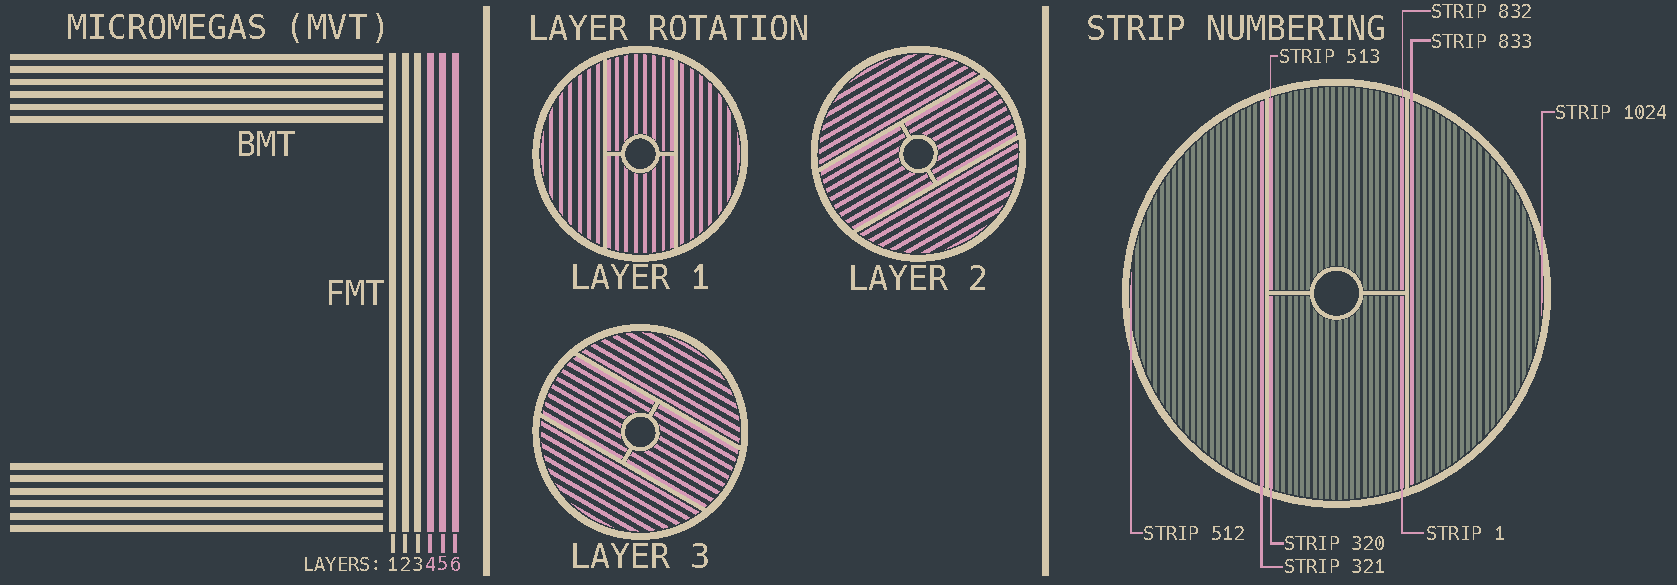
\includegraphics[width=0.98\linewidth]{02fmt_geometry.pdf}}
    \end{center}

    \backref{10.34::fmt}
\end{frame}
